\section{Code Transformation}\label{sec:trans}

%\subsection{Formalization of the Transformation Rules}
\subsection{Formalization of Transformation Rules}

% todo: graphical issue in this figure image
\begin{figure}[ht!]
	\begin{subfigure}{1\textwidth}
		\centering
		%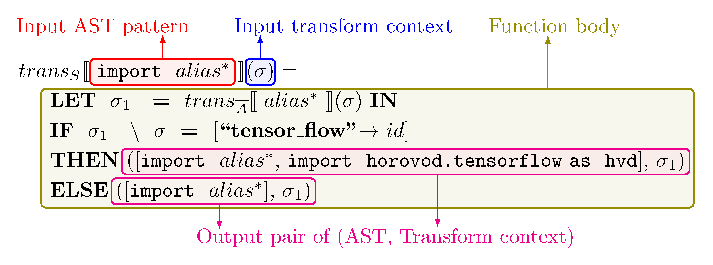
\includegraphics[width=0.8\textwidth]{Fig14.eps}
		\begin{lstlisting}[language=Python]
trans_S(`import {aliases}`, ctx):
  let ctx_1 = trans_A(`{aliases}`, ctx).context
  if diff(ctx_1, ctx) == ["tensorflow" -> `{id}`]:
    return (`import {aliases}; import horovod.tensorflow as hvd`, ctx_1)
  else:
    return (`import {aliases}`, ctx_1)
		\end{lstlisting}
		\caption{Transform function of import statements}
		\label{fig:trans:ex01:code}
	\end{subfigure}

    \begin{subfigure}[b]{0.4\textwidth}
        \begin{lstlisting}[language=Python]
import tensorflow as tf\end{lstlisting}
        \caption{Original DL python code}
        \label{fig:trans:ex01:org}
    \end{subfigure}
    ~
    % hvd
    \begin{subfigure}[b]{0.56\textwidth}
        \begin{lstlisting}[language=Python]
import tensorflow as tf
import horovod.tensorflow as hvd\end{lstlisting}
        \caption{Transformed DL python code}
        \label{fig:trans:ex01:hvd}
    \end{subfigure}

	\caption{Transform function example}
    \label{fig:trans:fnexpl}
\end{figure}

% new
\noindent
We formalize the rules for transforming single-GPU models into multi-GPU
models using pure functions called {\it transform functions}. 
\begin{inred}
Transform functions take a Python AST and a {\it context} object as inputs,
and return a Python AST and a context object as output.
A context object is a mapping from strings to Python identifier ASTs;
context objects store and propagate necessary identifiers.
This enables (pure) transform functions to pass relevant contextual information
to subsequent function calls and utilize the information from outside their
input AST.

Figure \ref{fig:trans:ex01:code} illustrate a pseudocode of an example 
transform function thats transforms an import statement.
The transform function {\tt trans\_S} gets an input AST and a context object.
In the pseudocode, we use back-quoted notation {\tt `import \{aliases\}`} 
to represent a Python AST object;
the brace-surrounded expression represents a child AST.
Line 2 creates a new context object by calling the transformation function
on the child AST, {\tt `\{aliases\}`}.
Then line 3 computes the difference between the original context object {\tt ctx}
and the new context object {\tt ctx\_1}.
If the new context additionally stores {\tt "tensorflow"} entry,
it means that the import statement imports the TensorFlow library,
so the transform function concatenates a new import statement
{\tt import horovod.tensorflow as hvd} to the input AST and returns it.
If else, the function returns the same AST, with the new context object.
\end{inred}

% These functions take ASTs as input and produce ASTs as output. 
% In addition, the functions use {\it transform context} objects to incorporate
% contextual information during the transformation process. 
% The transform context maps strings to identifiers, which stores and
% propagates necessary identifiers used for the transformation.
% Each transform function takes a transform context as an additional input, uses
% and updates it in the function body, and produces the updated transform context
% as an additional output.
% This enables transform functions to utilize contextual information outside
% their input ASTs and pass relevant contextual information to subsequent
% transform functions.
%We present the formalization of the transformation rules in terms of
%\textit{trasnform functions}.
%Transform functions are the pure functions from ASTs to ASTs.
%By applying the transform function to AST of the input single-GPU model,
%we can get the AST of the transformed multi-GPU model.
%Transform functions also receive and return objects called \textit{transform
%context} in order to utilize the contextual information during the 
%transformation process.
%The transform context is a finite mapping from strings to identifiers, which
%stores arbitrary identifiers from the code and propagate them to the 
%next transform function.
%When transform functions are sequentially applied to sequence of ASTs, 
%the output transform context from the previous call is given as the input
%to the next tranform function call.
%By this method, the transform functions can utilize contextual information
%outside of their input AST and propagate some contextual information from
%their input AST to next transform function calls.
%
% transform function format expl
% 이 파트를 어떻게 효과적으로 설명해야할지 확신이 안드는 상태
% We define the transform functions as a collection of partial transform
% functions, of which one example is illustrated in
% Figure~\ref{fig:trans:fnexpl}. 
% These partial functions operate only on ASTs that match a specified code
% pattern in the input AST parameter position. 
% Any input ASTs that do not match the pattern remain unmodified. 
% For example, the function in Figure~\ref{fig:trans:fnexpl} matches only {\tt
% import} statements and transforms them accordingly. 
% The function takes the transform context $\smodenv$ as an additional input, and
% its body produces a pair of the output expression and the updated transform
% context. 
% We use compound expressions such as {\tt LET-IN} and {\tt IF-THEN-ELSE} to
% specify different outputs depending on certain conditions. 
% In Figure~\ref{fig:trans:fnexpl}, the function body uses a {\tt LET-IN}
% expression to store the updated transform context by another transform function
% applied to the sub phrase $alias^*$ to $\sigma_1$. 
% Also, it uses an {\tt
% IF-THEN-ELSE} expression to return different results depending on whether the
% {\tt import} statement imports the {\tt tensorflow} module or not.
%
% \begin{figure}[ht!]
%     \centering
%     % org
%     \begin{subfigure}[b]{0.4\textwidth}
%         \begin{lstlisting}[language=Python]
% import tensorflow as tf\end{lstlisting}
%         \caption{Original DL python code}
%         \label{fig:trans:ex01:org}
%     \end{subfigure}
%     ~
%     % hvd
%     \begin{subfigure}[b]{0.56\textwidth}
%         \begin{lstlisting}[language=Python]
% import tensorflow as tf
% import horovod.tensorflow as hvd\end{lstlisting}
%         \caption{Transformed DL python code}
%         \label{fig:trans:ex01:hvd}
%     \end{subfigure}
%     \caption{Example code transformation result}
%     \label{fig:trans:ex01}
% \end{figure}
%
% Figure~\ref{fig:trans:ex01} shows the example code transformation result by the
% partial transform function in Figure~\ref{fig:trans:fnexpl}.
% Because the statement in Figure~\ref{fig:trans:ex01:org} is an import statement
% matched with the input AST pattern of the function, the function is responsible
% for transforming the statement.
% The function first computes the transform context $\smodenvsubs{1}$ that
% includes all the modules and their alias identifiers imported by the statement.
% Next, the function calculates the difference between $\smodenvsubs{1}$ and the
% input transform context $\smodenv$.
% Suppose the difference contains the new entry for the string {\tt "tensor\_flow"}.
% In that case, the transform function returns a statement list containing the
% original statement and a new statement {\tt import horovod.tensorflow as hvd}
% to add the import statement for the {\tt horovod} module after the original
% statement, as shown in Figure~\ref{fig:trans:ex01:hvd}.  
% Otherwise, the function returns a statement list containing only the original
% statement remaining unchanged.
The following subsection briefly presents essential code transform rules for
each training API pattern with formal descriptions. 
We also provide the full formal transform rules as a companion
report~\footnote{https://github.com/kaist-plrg/python-analyzer/blob/main/trans/trans.pdf}.

%We describe the transform function as the collection of the partial transform
%function. 
%The figure~\ref{fig:trans:fnexpl} illustrates an example of the
%partial transform function.
%We use the AST pattern in the input parameter position.
%The input AST pattern means that the partial function only applies
%to the input ASTs that match the pattern.
%The input ASTs taht does not match the pattern will not be modified.
%For instance, the function in the figure~\ref{fig:trans:fnexpl} only matches
%the {\tt import} statements and transform them. 
%The function also takes the transform context $\smodenv$ as an input.
%The function body defines the output expression. 
%We use complex expressions such as {\tt LET-IN} or {\tt IF-THEN-ELSE} to 
%check and specify conditions to return different outputs.
%In the figure~\ref{fig:trans:fnexpl}, 
%the function body uses {\tt IF-THEN-ELSE} expression to check if the 
%{\tt import} statement imports the {\tt tensorflow} module, 
%and returns different ASTs according to the condition.

%\pagebreak
%\begin{figure}[ht!]
%  \centering
%  \begin{subfigure}[t]{0.48\textwidth}
%    \begin{lstlisting}[language=Python]
%import tensorflow as tf
%
%dataset = ...
%model = ...
%optim = tf.optimizers.Adam(0.001) 
%
%for (x, y) in dataset.take(10000):
%  with tf.GradientTape() as tape:
%    pred = model(x)
%    loss_value = loss(y, pred)\end{lstlisting} 
%    \caption{Original DL training code}
%  \end{subfigure}
%  \hspace{5mm}
%  \begin{subfigure}[t]{0.48\textwidth}
%    \begin{lstlisting}[language=Python]
%import tensorflow as tf
%import horovod.tensorflow as hvd
%
%dataset = ...
%model = ...
%optim = tf.optimizers.Adam(0.001 * hvd.size()) 
%
%for (x, y) in dataset.take(10000):
%  with tf.GradientTape() as tape:
%    pred = model(x)
%    loss_value = loss(y, pred) 
%  tape = hvd.DistributedGradientTape(tape)\end{lstlisting}
%    \caption{Distributed DL training code}
%  \end{subfigure}
%  \caption{Example of original DL model code transformed into the distributed model}
%  \label{fig:trans:ex}
%\end{figure}
%
%We explain how transform functions are defined to transform the DL model codes
%in the example in figure \ref{fig:trans:ex}.
%Figure \ref{fig:trans:ex} is an example of single-GPU model code and
%the corresponding distributed model code.
%There are three transformed parts of the code. 
%First, an import statement for the {\tt horovod} module is added in the line 2. 
%The statement is added right after the {\tt tensorflow} module import statement.
%Second, in the line 6, the argument of the {\tt Optimizer} instance constructor
%is modified. The new argument expression multiplies {\tt hvd.size()} 
%to the original argument expression.
%Third, in the line 12, an assign statement is added. 
%The assignment wraps the original {\tt GradientTape} object with
%the Horovod library function, {\tt hvd.DistributedGradientTape}.

%\begin{figure}[ht!]
%    \centering
%    % org
%    \begin{subfigure}[b]{0.48\textwidth}
%        \begin{lstlisting}[language=Python]
%import tensorflow as tf\end{lstlisting}
%        \caption{Original DL training code: only TensorFlow module is imported.}
%        \label{fig:trans:ex01:org}
%    \end{subfigure}
%    ~
%    % hvd
%    \begin{subfigure}[b]{0.48\textwidth}
%        \begin{lstlisting}[language=Python]
%import tensorflow as tf
%import horovod.tensorflow as hvd\end{lstlisting}
%        \caption{Distributed DL training code: Horovod module import statement is added.}
%        \label{fig:trans:ex01:hvd}
%    \end{subfigure}
%    % fn
%    \begin{subfigure}[t]{\textwidth}
%        \centering
%        \begin{tabular}{l}
%            \typdesc{\fkstmt& : & \dstmt ~ $\rightarrow$ ~ \dmodenv ~ 
%            $\rightarrow$ ~ (\dstmt ~ list ~ $\times$ ~ \dmodenv)}\\
%            \tstmt{\kimport ~ \mul{\nalias}}{\smodenv} = \\
%            \inden \ktlet ~ \smodenvsubs{1} ~ \kteq ~ \taalias{\mul{\nalias}}{\smodenv} \ktin \\
%            \inden \ktif ~ \smodenvsubs{1} ~ \envsub ~ \smodenv ~ \kteq ~ [\tflow $\mapsto$ \nid]\\ 
%            \inden\ktthen \\
%            \inden\hspace{1em} ([\kimport ~ \mul{\nalias},
%            \kimport ~ {\tt horovod.tensorflow} \kas ~ {\tt hvd}], \smodenvsubs{1})\\
%            \inden \ktelse~([\kimport ~ \mul{\nalias}], \smodenvsubs{1})
%\end{tabular}\\\vpar
%
%        \caption{The Partial Transform function}
%        \label{fig:trans:ex01:fn}
%    \end{subfigure}
%
%    \caption{Transformation of Adding the Horovod {\tt import} Statement}
%    \label{fig:trans:ex01}
%\end{figure}


%Figure \ref{fig:trans:ex01} describes the partial transform function that
%transforms the first part of the code.
%The input AST pattern matches an import statement that imports the
%{\tt tensorflow} module.
%The line 2 in the figure~\ref{fig:trans:ex01:fn} first computes the
%$\smodenvsubs{1}$, which is the transfom context that includes the modules 
%imported by the input statement.
%Then the line 3 compute the difference between $\smodenvsubs{1}$ 
%and the input transform context $\smodenv$.
%If the difference includes the new entry for string {\tt "tensor\_flow"},
%it means that the import statement imports the {\tt tensorFlow} module.
%In this case, the transform function adds the {\tt horovod} module import 
%statement after the original statement.
%
%\pagebreak
%\begin{figure}[ht!]
%    \centering
%
%    \begin{subfigure}[t]{0.48\textwidth}
%        \begin{lstlisting}[language=Python]
%        optim = tf.optimizers.Adam(0.001)\end{lstlisting}
%        \caption{Original DL training code}
%    \end{subfigure}
%
%    \hspace{5mm}
%
%    \begin{subfigure}[t]{0.48\textwidth}
%        \begin{lstlisting}[language=Python]
%        optim = tf.optimizers.Adam(0.001 * hvd.size())\end{lstlisting}
%        \caption{Distributed DL training code}
%    \end{subfigure}
%
%    \begin{subfigure}[t]{\textwidth}
%        \centering
%        \begin{tabular}{l}
%
%            \typdesc{\fkstmt& : & \dstmt ~ $\rightarrow$ ~ \dmodenv ~ $\rightarrow$ ~ (\dstmt ~ list ~ $\times$ ~ \dmodenv)}\\
%
%            \tstmt{\nidsubs{r} \oassign \nexprsubs{1} \sparen{\nexprsubs{11} ... \nexprsubs{1n}} }{\smodenv} = \\
%
%            \inden \ktif ~ \nexprsubs{1} \ktsubtysubs{\smodenv} ~ {\tt tensorflow.keras.optimizers.Optimizer}\\
%            \inden \ktthen \\
%
%            \inden\inden ([\nidsubs{r} \oassign \nexprsubs{1} \sparen{\nexprsubs{11}
%            {\tt * hvd.size()} ... \nexprsubs{1n}}], \smodenv[\optmizer $\mapsto$ \nidsubs{r}])\\
%
%        \end{tabular}
%        \caption{Transform function: scaling the Optimizer instance argument}
%        \label{fig:trans:fn02}
%    \end{subfigure}
%    \caption{Code examples}
%    \label{fig:trans:ex02}
%\end{figure}
%
%Figure \ref{fig:trans:ex02} the transform function that transformed the second
%part of the code.
%The learning rate argument for the {\tt Optimizer} class constructor is 
%multiplied by the expression {\tt hvd.size()}. 
%To apply the transformation, the transform function must first recognize a
%assign statement that creates an {\tt Optimizer} instance.
%One caveat here is that the {\tt Optimizer} instance can be 
%created by not only TensorFlow library APIs, but also
%user-defined class constructors. 
%The transform function utilizes the class inheritance information
%generated by the class hierarchy analyzer to recognize the user-defined
%constructors for {\tt Optimizer} subclasses.
%
%After identifying the {\tt Optimizer} instance assign statement, 
%the transform function modifies the argument expression of the
%constructor call.
%The transform function would take the original argument expression,
%then create a new expression that multiplies {\tt hvd.size()}
%To modify the argument expression, the function body utilizes the AST pattern
%variable $\nexprsubs{11}$ in the input AST pattern.
%The pattern variable $\nexprsubs{11}$ will match {\tt 0.001} in the figure
%\ref{fig:trans:ex02}(a).
%In the output AST, the modified argument expression 
%$\nexprsubs{11} {\tt * hvd.size()}$ will expand to {\tt 0.001 * hvd.size()}.
%
%\begin{figure}[ht!]
%  \centering
%  \begin{subfigure}[t]{0.48\textwidth}
%    \begin{lstlisting}[language=Python]
%for (x, y) in dataset.take(10000):
%  with tf.GradientTape() as tape:
%    pred = model(x)
%    loss_value = loss(y, pred)\end{lstlisting} 
%    \caption{Original DL training code}
%  \end{subfigure}
%  \hspace{5mm}
%  \begin{subfigure}[t]{0.48\textwidth}
%    \begin{lstlisting}[language=Python]
%for (x, y) in dataset.take(10000):
%  with tf.GradientTape() as tape:
%    pred = model(x)
%    loss_value = loss(y, pred) 
%  tape = hvd.DistributedGradientTape(tape)\end{lstlisting}
%    \caption{Distributed DL training code}
%  \end{subfigure}
%  \caption{Example of original DL model code transformed into the distributed model}
%  \label{fig:trans:ex03}
%\end{figure}
%
%\begin{figure}[ht!]
%  \centering
%  \begin{tabular}{l}
%  \typdesc{\fkstmt& : & \dstmt ~ $\rightarrow$ ~ \dmodenv ~ $\rightarrow$ ~ (\dstmt ~ list ~ $\times$ ~ \dmodenv)}\\
%  \tstmt{\kwith ~ \mul{\nwithitem} ~ \kcolon ~ \mul{\nstmt}}{\smodenv} = \\
%  \inden \ktlet ~ \mul{\nwithitem}$'$, \smodenvsubs{1} \kteq ~ \twwithitem{\mul{\nwithitem}}{\smodenv} \ktin \\
%  \inden \ktlet ~ \mul{\nstmt}$'$, \smodenvsubs{2} \kteq ~ \tsstmt{\mul{\nstmt}}{\smodenvsubs{1}} \ktin \\
%  \inden \ktif ~ \smodenvsubs{1} \envsub ~ \smodenv ~ \kteq ~ [\gtape $\mapsto$ \nid] ~ \ktthen\\
%  \inden\inden ([\kwith ~ \mul{\nwithitem}$'$ ~ \kcolon ~ \mul{\nstmt}$'$, \\
%  \inden\inden \nid ~ \oassign {\tt hvd.DistributedGradientTape(\nid)}], \smodenvsubs{2})\\
%  \inden \ktelse ~ ([\kwith ~ \mul{\nwithitem}$'$ ~ \kcolon ~ \mul{\nstmt}$'$], \smodenvsubs{2})
%\end{tabular}\\\vpar
%  \caption{Transform function: wrapping GraidentTape instance with Horovod API}
%  \label{fig:trans:fn03}
%\end{figure}
%
%Figure \ref{fig:trans:ex03} describes the transform function that transforms
%the third part of the code.
%An assign statement is added after the {\tt with} statement body end.
%To apply this transformation, the transform function must first identify
%a with statement that creates a {\tt GradientTape} instance. 
%The transform function utilizes the transform context to recognize whether a
%with statement creates a new {\tt GradientTape} instance or not. 
%The transform function compares the input transform context with the 
%transform context just after processing the with statement to check
%whether the input with statement creates a {\tt GradientTape} instance.
%Then, the transform function adds a new assign statement after the 
%with statement, which wraps the variable with a
%{\tt DistributedGradientTape} Horovod API.

% next subsection
\subsection{Transformation Rules for API Patterns}

%As mentioned earlier, different API patterns of the codes
%require different transformation rules to correctly transform them.
%To apply different transformation rules for different API pattern codes,
%we defined sets of transform functions each for trainng API patterns.
%This section explains the transform functions defined for each API patterns.

\subsubsection{Rules for the Session Pattern}

\begin{figure}[ht!]\centering
  \begin{subfigure}[t]{0.9\textwidth}
    \begin{lstlisting}[style=mpython]
optimizer = tf.train.MomentumOptimizer(learning_rate = 0.01)

with tf.Session() as sess:
    for step in range(num_epochs): 
        sess.run(optimizer, feed_dict)\end{lstlisting}
    \caption{Session pattern example}
    \label{fig:trans:sessiontrans:a}
  \end{subfigure}
  \hspace{5mm}
  \begin{subfigure}[t]{0.9\textwidth}
    \begin{lstlisting}[style=mpython]
optimizer = tf.train.MomentumOptimizer(learning_rate = 0.01 * hvd.size())
optimizer = hvd.DistributedOptimizer(optimizer)

with tf.Session() as sess:
    for step in range(num_epochs): 
        sess.run(optimizer, feed_dict)\end{lstlisting}
    \caption{Distributed Session pattern example}
    \label{fig:trans:sessiontrans:b}
  \end{subfigure}
  \caption{Example transformation of the Session pattern}
  \label{fig:trans:sessiontrans}
\end{figure}

\noindent
Figure \ref{fig:trans:sessiontrans} illustrates the required transformation of
the Session pattern using two code examples, \ref{fig:trans:sessiontrans:a} the
original training code and \ref{fig:trans:sessiontrans:b} its distributed
training version.
One of the primary transformations involves adjusting the learning rate
argument in the {\tt Optimizer} constructor call, which is achieved by
multiplying it by the number of GPUs.
The learning rate can be passed as the first positional argument in the
constructor call or as the keyword argument {\tt learning\_rate}.
The other transformation uses the Horovod-provided {\tt DistributedOptimizer}
instance instead of the original {\tt Optimizer} instance. 
To create the {\tt DisributedOptimizer} instance, the original {\tt Optimizer}
is passed as an argument to its constructor.

%To correctly transform Session pattern training codes into distributed 
%training codes, the {\tt Optimizer} instance must be modified.
%Figure \ref{fig:trans:sessiontrans} shows a pair of code examples
%illustrating the required transformation for Session pattern case.
%In line 1 of figure \ref{fig:trans:sessiontrans}(b),
%the learning rate argument is scaled by {\tt hvd.size()}.
%The learning rate can be specified by keyword argument {\tt learning\_rate}
%as the figure \ref{fig:trans:sessiontrans},
%or by the first positional argument.
%The transform function should be able to transform both of the cases.
%The transformation also adds a new statementd that wraps the 
%{\tt Optimizer} instance by {\tt DistributedOptimizer}.

\begin{figure}[ht!]\small
\noindent
  \begin{tabularx}{\textwidth}{X}
  \tstmt{\nidsubs{r} \oassign \nexprsubs{1} \sparen{\nexprsubs{11} ... \nexprsubs{1n} ~ \op{(\nidsubs{1} \oassign)} \nexprsubs{21} ... \op{(\nidsubs{k} \oassign)} \nexprsubs{2k}} }{\smodenv} = \\
  \inden \ktif ~ \nexprsubs{1} \ktsubtysubs{\smodenv} ~ {\tt tensorflow.keras.optimizers.Optimizer} ~ \ktthen\\
  \inden\inden \ktif ~ \nidsubs{i} ~ \kteq ~ {\tt learning\_rate} ~ \ktwhen ~ 1 $\leq$ i $\leq$ k ~ \ktthen\\
  \inden\inden\inden ([\nidsubs{r} \oassign \nexprsubs{1} \sparen{\nexprsubs{11} ... \nexprsubs{1n} ~ \op{(\nidsubs{1} \oassign)} \nexprsubs{21} ... \nidsubs{i} \oassign \nexprsubs{2i} {\tt * hvd.size()}\\
  \inden\inden\inden\inden ... \op{(\nidsubs{k} \oassign)} \nexprsubs{2k}}, \\
  \inden\inden\inden {\tt \nidsubs{r} = hvd.DistributedOptimizer(\nidsubs{r})}],\\
  \inden\inden\inden \smodenv[\optmizer $\mapsto$ \nidsubs{r}])\\

  \inden\inden \ktelse \\
  \inden\inden\inden ([\nidsubs{r} \oassign \nexprsubs{1} \sparen{\nexprsubs{11} {\tt * hvd.size()}... \nexprsubs{1n} ~ \op{(\nidsubs{1} \oassign)} \nexprsubs{21} ... \nidsubs{i} \oassign \nexprsubs{2i}\\
  \inden\inden\inden\inden ... \op{(\nidsubs{k} \oassign)} \nexprsubs{2k}}, \\
  \inden\inden\inden {\tt \nidsubs{r} = hvd.DistributedOptimizer(\nidsubs{r})}], \\
  \inden\inden\inden\smodenv[\optmizer $\mapsto$ \nidsubs{r}])\\

\end{tabularx}
  \caption{Session pattern transform function: Optimizer learning rate scaling and wrapping}
  \label{fig:trans:sessrule}
\end{figure}

Figure \ref{fig:trans:sessrule} shows the essential rule for the Session pattern,
which conducts the two transformations.
The transform rule matches an assignment statement that stores the result of a
function call expression into a variable.
Initially, the rule examines whether the callee function is the constructor of
either the {\tt Optimizer} class or any of its subclasses.
The predicate \ktsubtysubs{\smodenv} checks the subclass relation between two
classes using the class hierarchy analysis result.
Then, the rule adjusts the learning rate argument of the constructor call. 
Suppose the learning rate is passed as a keyword argument. 
In that case, the rule replaces the keyword argument value with the
multiplication of the original learning rate and the return value of {\tt
horovod.size()}.
Otherwise, the rule adjusts the first argument instead.
Following the adjustment of the learning rate, the rule adds a new statement:
$id_r\ =\ ${\tt hvd.DistributedOptimizer($id_r$)}. 
This statement replaces the original optimizer instance with a distributed
optimizer instance for any subsequent uses.

%Figure \ref{fig:trans:sessrule} formalizes the Sesison pattern transform 
%function. The transform function 
%matches assign statements that assign a result of function call expression.
%If an assign statement is matched, the pattern guard checks if the
%callee function is the {\tt Optimizer} instance constructor function.
%The pattern guard uses the subclass predicate \ktsubtysubs{\smodenv}
%to identify any expression that constructs the subclass of the TensorFlow
%{\tt Optimizer} class including user-defined classes.

%The third line of the transform function uses a branch to distinguish 
%whether the {\tt learning\_rate} argument is given as a keyword argument or not. 
%When the argument is given as a keyword argument,
%the transform function modifies the corresponding keyword argument expression
%as shown in the true branch in fourth line.
%When the argument is not given as a keyword argument,
%the transform function assumes that the first positional argument
%is the {\tt learning\_rate} argument and modifies it
%as shown in the eighth line.
%In either case, the transform function additionally returns a new
%assign statement that wraps the {\tt Optimizer} with
%{\tt hvd.DistributedOptimizer}.

\subsubsection{Rules for the MonitoredSession Pattern}
Figure~\ref{fig:trans:monsesstrans} describes an example transformation of the
MonitoredSession pattern code.
The {\tt MonitoredSession} constructor optionally requires a list of {\tt
SessionRunHook} objects as a keyword argument {\tt hooks}.
To ensure consistent global variable initialization of all processes in the
distributed training, the list needs to contain a {\tt
BroadcastGlobalVariableHook} object for the global variable broadcasting, as
shown in Figure~\ref{fig:trans:monsesstrans:b}.
The instance can be created by calling the constructor of the {\tt
BroadcastGlobalVariableHook} class with the ID of a source process.  
When starting the training, the hook broadcasts the initial global variable
parameters of the source to the other processes.\\

\begin{figure}
  \centering
  \begin{subfigure}[t]{0.8\textwidth}
    \begin{lstlisting}[style=mpython]
with tf.train.MonitoredTrainingSession(hooks=hooks) as mon_sess:
    while not mon_sess.should_stop():
        mon_sess.run()\end{lstlisting}
    \caption{MonitoredSession pattern example}
    \label{fig:trans:monsesstrans:a}
  \end{subfigure}
  \hspace{5mm}
  \begin{subfigure}[t]{0.8\textwidth}
    \begin{lstlisting}[style=mpython]
with tf.train.MonitoredTrainingSession(hooks=hooks.append(hvd.BroadcastGlobalVariablesHook(0)) as mon_sess:
    while not mon_sess.should_stop():
        mon_sess.run()\end{lstlisting}
    \caption{Distributed MonitoredSession pattern example}
    \label{fig:trans:monsesstrans:b}
  \end{subfigure}
  \caption{Example transformation of the MonitoredSession pattern}
  \label{fig:trans:monsesstrans}
\end{figure}


%\newpage
%To correctly transform the MonitoredSesion pattern code with the Horovod
%framework, 
%a hook for the variable broadcasting should be added to the
%{\tt MonitoredSession} object. 
%As in figure \ref{fig:trans:monsesstrans}, for example,
%the transformation appends {\tt BroadcastGlobalVariablesHook} to the
%{\tt hooks} arguments of the {\tt MonitoredSession} constructor call.
\vspace{-1em}

\begin{figure}[ht!]\small
 \noindent
  \begin{tabular}{l}
    %\typdesc{\fkstmt& : & \dstmt ~ $\rightarrow$ ~ \dmodenv ~ $\rightarrow$ ~ (\dstmt ~ list ~ $\times$ ~ \dmodenv)} \\
    \tstmt{\kwith ~ \mul{\nwithitem} ~ \kcolon ~ \mul{\nstmt}}{\smodenv} = \\
    \inden \ktlet ~ \mul{\nwithitem}$'$, \smodenvsubs{1} \kteq ~ \twwithitem{\mul{\nwithitem}}{\smodenv} \ktin \\
    \inden \ktlet ~ \mul{\nstmt}$'$, \smodenvsubs{2} \kteq ~ \tsstmt{\mul{\nstmt}}{\smodenvsubs{1}} \ktin \\

    \inden ([\kwith ~ \mul{\nwithitem}$'$ ~ \kcolon ~ \mul{\nstmt}$'$], \smodenvsubs{2})
  \end{tabular}\\[2ex]

  \begin{tabular}{l}
    %\typdesc{\fkwithitem & : & \dwithitem ~ $\rightarrow$ ~ \dmodenv ~ $\rightarrow$ ~ (\dwithitem ~ $\times$ \dmodenv)}  \\
    \twithitem{\nexprsubs{1} \sparen{\nexprsubs{11} ... \nexprsubs{1n} ~ 
                \op{(\nidsubs{1} \oassign)} \nexprsubs{21} ... 
                \op{(\nidsubs{k} \oassign)} \nexprsubs{2k}} {\tt as} \nidsubs{as} }{\smodenv} = \\

    \inden \ktif ~ \nexprsubs{1} \ktsubtysubs{\smodenv} {\tt tensorflow.train.MonitoredSession} ~ \ktthen \\
    \inden\inden \ktif ~ \nidsubs{i} ~ \kteq ~ {\tt hooks} ~ \ktwhen ~ 1 $\leq$ i $\leq$ k ~ \ktthen\\
    \inden\inden\inden(\nexprsubs{1} \sparen{\nexprsubs{11} ... 
              \nexprsubs{1n} ~ \op{(\nidsubs{1} \oassign)} \nexprsubs{21} \\
    \inden\inden\inden\inden ... \nidsubs{i} \oassign {\tt \nexprsubs{2i}.append(hvd.BroadcastGlobalVariablesHook(0))} \\
    \inden\inden\inden\inden ... \op{(\nidsubs{k} \oassign)} \nexprsubs{2k} }, \\
    \inden\inden\inden\inden \smodenv[ \msess $\mapsto$ \nidsubs{as}]) \\
  \end{tabular}\\\vpar
\caption{MonitoredSession pattern transform function: Modifying {\tt StopAtStepHook} instance}
  \label{fig:trans:monsessrule}
\end{figure}

%\vspace{-1em}

Figure \ref{fig:trans:monsessrule} formalizes the transform functions for the
MonitoredSession pattern.
The first transform function is responsible for matching {\tt with} statements
and transforming a list of the {\tt with\_item}, each of which represents a
variable and an assigned expression. 
The transform function denoted as \fkwwithitem~in line 2 applies the second
transform function \fkwithitem~to each {\tt with\_item}.
As a result, the first transform function returns a new {\tt with} statement
containing a list of the transformed {\tt with\_item}.
The second transform function transforms the {\tt with\_item}.
Among many forms of the {\tt with\_item}, the function matches those that
assign a function call result to a variable.
The second line checks whether the callee function of the {\tt with\_item} is a
constructor of the subclass of the {\tt MonitoredSession} class. 
If then, the transform function finds the keyword argument {\tt hooks} and
appends a {\tt BroadcastGlobalVariablesHook} object to the argument.\\

\subsubsection{Rules for the GradientTape pattern}\label{sec:grad}

\begin{figure}[ht!]
  \centering
  \begin{subfigure}[t]{0.8\textwidth}
    \begin{lstlisting}[style=mpython]
import tensorflow as tf

with tf.GradientTape() as tape:
    probs = model(images)
    loss_value = loss(labels, probs)

grads = tape.gradient(loss_value, model.trainable_variables)
opt.apply_gradients(zip(grads, model.trainable_variables))\end{lstlisting}
    \caption{GradientTape pattern example}
    \label{fig:trans:gtapetrans:a}
  \end{subfigure}
  \hspace{5mm}
  \begin{subfigure}[t]{0.8\textwidth}
    \begin{lstlisting}[style=mpython]
import tensorflow as tf
import horovod.tensorflow as hvd
hvd_broadcast_done = False

with tf.GradientTape() as tape:
    probs = model(images)
    loss_value = loss(labels, probs)
tape = hvd.DistributedGradientTape(tape)
grads = tape.gradient(loss_value, model.trainable_variables)
id_new = zip(grads, model.trainable_variables)
opt.apply_gradients(id_new)

global hvd_broadcast_done
if not hvd_broadcast_done:
    hvd.broadcast_variables([x[1] for x in id_new], root_rank=0,)
    hvd.broadcast_variables(opt.variables(), root_rank=0,)
    hvd_broadcast_done = True\end{lstlisting}
    \caption{Distributed GradientTape pattern example}
    \label{fig:trans:gtapetrans:b}
  \end{subfigure}
  \caption{Example transformation of the GradientTape pattern}
  \label{fig:trans:gtapetrans}
\end{figure}

\noindent
Figure \ref{fig:trans:gtapetrans} illustrates an example GradientTape pattern
code and its distributed version.  
For the distributed training, the model needs to utilize a {\tt
DistributedGradientTape} instance in training instead of the {\tt
GradientTape} instance, as shown in lines 8 and 9 in
Figure~\ref{fig:trans:gtapetrans:b}.
In addition, the model also needs to broadcast trainable global variables from
the root process to the others once after applying the gradients.
Lines 13 to 17 in Figure~\ref{fig:trans:gtapetrans:b} represent the code that
broadcasts the variables depending on the value of {\tt hvd\_broadcast\_done}.
Once finishing the broadcasting, the {\tt hvd\_broadcast\_done} is set to {\tt
False} to prevent further broadcasting.

%To correctly transform GradientTape pattern training codes,
%the {\tt GradientTape} instance should be modified for distributed training.
%As shown in line 8, figure \ref{fig:trans:gtapetrans}(b),
%the {\tt GradientTape} instance {\tt tape}
%is wrapped by a Horovod library API {\tt DistributedGradientTape}.
%In addition to modifying the {\tt GradientTape} instance,
%lines 13 to 17 add the variable broadcasting code after the
%{\tt apply\_gradients} method call.
%Note that the variable {\tt hvd\_broadcast\_done} is initialized as 
%{\tt False} at line 3. 
%Then line 17 sets the variable to {\tt True}, after the variable broadcasting
%is done.
%We use the boolean variable {\tt hvd\_broadcast\_done} in GrdientTape pattern
%model to ensure that variable broadcasting occurs exactly once.


\begin{figure}[ht!]\small
%\noindent
\begin{tabular}{l}
  \tstmt{\kwith ~ \mul{\nwithitem} ~ \kcolon ~ \mul{\nstmt}}{\smodenv} = \\
  \inden \ktlet ~ \mul{\nwithitem}$'$, \smodenvsubs{1} \kteq ~ \twwithitem{\mul{\nwithitem}}{\smodenv} \ktin \\
  \inden \ktlet ~ \nstmt$'$, \smodenvsubs{2} \kteq ~ \tsstmt{\mul{\nstmt}}{\smodenvsubs{1}} \ktin \\
  \inden \ktif ~ \smodenvsubs{1} \envsub ~ \smodenv ~ \kteq ~ [\gtape $\mapsto$ \nid] ~ \ktthen\\
  \inden\inden ([\kwith ~ \mul{\nwithitem}$'$ ~ \kcolon ~ \mul{\nstmt}$'$, \nid ~ \oassign {\tt hvd.DistributedGradientTape(\nid)}], \smodenvsubs{2})\\
  \inden \ktelse ~ ([\kwith ~ \mul{\nwithitem}$'$ ~ \kcolon ~ \mul{\nstmt}$'$], \smodenvsubs{2})
\end{tabular}
  \caption{GradientTape pattern transform function: utilizing the {\tt DistributedGradientTape} instance}
  \label{fig:trans:gtaperule}
\end{figure}

Figure \ref{fig:trans:gtaperule} formalizes the partial transform function for
utilizing the {\tt DistributedGradientTape} instance.
The transform function matches {\tt with} statements and updates the transform
context by transforming the list of {\tt with\_item}.
The updated transform context contains a mapping from the string {\tt
graident\_tape} to a variable \nid~if the {\tt with\_item} creates a {\tt
GradientTape} instance and assigns it to the variable.
Then, the function injects a new assignment statement, $\nid ~ \oassign~{\tt
hvd.DistributedGradientTape(\nid)}$, right after the {\tt with} statement,
which replaces the instance of the variable with a newly created {\tt
DistributedGradientTape} instance for further uses in subsequent statements.


\begin{figure}[ht!]\small
\noindent
\begin{tabular}{l}
  \tstmt{\nidsubs{r} \oassign \nexprsubs{1} \sparen{\nexprsubs{11} ... \nexprsubs{1n} ~ \op{(\nidsubs{1} \oassign)} \nexprsubs{21} ... \op{(\nidsubs{k} \oassign)} \nexprsubs{2k}} }{\smodenv} = \\
  \inden \ktif  ~ \smodenv(\optmizer) ~ \kteq ~ \nidsubs{t} ~ \ktand ~ \nexprsubs{1} ~ \kteq ~ {\tt \nidsubs{t}.apply\_gradients} ~ \ktthen\\
  \inden\inden \ktlet ~ \nidsubs{z} ~ \kteq ~ \newid ~ \ktin \\
  \inden\inden ([\nidsubs{z} ~ \oassign ~ \nexprsubs{11},\\
  \inden\inden \nidsubs{r} \oassign \nexprsubs{1} \sparen{\nidsubs{z} \nexprsubs{12} ... \nexprsubs{1n} ~ \op{(\nidsubs{1} \oassign)} \nexprsubs{21} ... \op{(\nidsubs{k} \oassign)} \nexprsubs{2k}} ,\\
  \inden\inden {\tt global hvd\_braodcast\_done},\\
  \inden\inden {\tt if not hvd\_broadcast\_done:} \\ 
  \inden\inden\inden [ {\tt hvd.broadcast\_variables([x[1] for x in \nidsubs{z}], root\_rank=0)}, \\
  \inden\inden\inden {\tt hvd.broadcast\_variables(\nidsubs{t}.variables(), root\_rank=0)}, \\
  \inden\inden\inden {\tt hvd\_broadcast\_done = True} ]\\
  \inden\inden ], \smodenv) \\
\end{tabular}
  \caption{GradientTape pattern transform function: broadcasting trainable global variables}
  \label{fig:trans:gtaperule2}
\end{figure}

Figure \ref{fig:trans:gtaperule2} formalizes the partial transform function
that appends the variable broadcasting code after the 
{\tt apply\_gradients} method call.
The function matches assignment statements that assign a function call result. 
When a variable $id_t$ stores the {\tt Optimizer} instance and the callee
function is {\tt $id_t$.apply\_gradients}, the transform function changes the
assignment statement and adds the variable broadcasting code.
The function injects a new assignment statement that stores the first argument
of the function call into a new variable $id_z$.
The first argument of the {\tt apply\_gradients} is an iterator of tuples that
contain pairs of gradients and trainable variables.
After the function call statement, the transform function injects a {\tt
global} statement to refer to the global broadcast flag variable {\tt
hvd\_broadcast\_done} and call statements guarded by the flag to broadcast
trainable variables stored in the tuples and {\tt opt.variables()}. 
The function also injects an assignment statement that sets the
global broadcast flag to {\tt True}.

%\pagebreak

   


\subsubsection{Rules for the Keras pattern}

\begin{figure}[ht!]\centering
  \begin{subfigure}[t]{0.8\textwidth}
  \begin{lstlisting}[style=mpython]
class ResNet(keras.Model):
    def __init__(self, block_list):
        ...

model = ResNet([2, 2, 2])

model.fit(x_train, y_train)\end{lstlisting}
  \caption{Keras pattern example}
    \label{fig:trans:keras:a}
  \end{subfigure}
  \hspace{3mm}
  \begin{subfigure}[t]{0.8\textwidth}
  \begin{lstlisting}[style=mpython]
class ResNet(keras.Model):
    def __init__(self, block_list):
        ...

model = ResNet([2, 2, 2])

callbacks=[hvd.callbacks.BroadcastGlobalVariablesCallback(0)]
model.fit(x_train, y_train,
          callbacks=callbacks)\end{lstlisting}
    \caption{Distributed Keras pattern example}
    \label{fig:trans:keras:b}
  \end{subfigure}
  \caption{Example transformation of the Keras Pattern}
  \label{fig:trans:keras}
\end{figure}

\noindent
Figure \ref{fig:trans:keras} illustrates an example transformation of the Keras
pattern.
The Keras pattern code usually defines a subclass of {\tt keras.Model}, such
as {\tt ResNet}, constructs a model as an instance of the class, and trains the
model by calling its {\tt fit} method inherited from {\tt keras.Model}.
To distribute the model's training with Horovod, the {\tt fit} method needs to
take a callback {\tt BroadcastGlobalVariablesCallback} as the keyword argument
{\tt callbacks}, shown in Figure~\ref{fig:trans:keras:b}.
When training starts, the callback ensures consistent initialization of all
processes by broadcasting initial global variable states from a source to the
other processes.

\begin{figure}[ht!]\small
\centering
\begin{tabular}{l}
  \tstmt{\nexprsubs{1} \sparen{\nexprsubs{11} ... \nexprsubs{1n} ~ \op{(\nidsubs{1} \oassign)} \nexprsubs{21} ... \op{(\nidsubs{k} \oassign)} \nexprsubs{2k}}}{\smodenv} = \\
  \inden \ktif ~ \nidsubs{m} ~ \kteq ~ \smodenv({\tmodel}) ~ \ktand ~ 
          \nexprsubs{1} ~ \kteq ~ {\tt \nidsubs{m}.fit} ~ \ktthen \\
  \inden\inden \ktif ~ \nidsubs{i} ~ \kteq ~ {\tt callbacks} ~ \ktwhen ~ 2 $\leq$ i $\leq$ k ~ \ktthen \\
  \inden\inden\inden ([{\tt cb = [hvd.callbacks.BroadcastGlobalVariablesCallback(root\_rank=0)},\\
  \inden\inden\inden ~ {\tt if hvd.rank() == 0: cb.append(\nexprsubs{2i})}, \\
  \inden\inden\inden ~ {\tt \nexprsubs{1} (\nexprsubs{11} ... \nexprsubs{1n}}
                              \op{(\nidsubs{1} \oassign)} \nexprsubs{21} ... 
                              \nidsubs{i} \oassign {\tt cb} ... 
                              \op{(\nidsubs{k} \oassign)} \nexprsubs{2k}{\tt )}], \smodenv) \\
  \inden\inden \ktelse \\
  \inden\inden\inden ([{\tt cb = [hvd.callbacks.BroadcastGlobalVariablesCallback(root\_rank=0)},\\
  \inden\inden\inden ~ {\tt \nexprsubs{1} (\nexprsubs{11}... \nexprsubs{1n}}
                              \op{(\nidsubs{1} \oassign)} \nexprsubs{21} ... 
                              \op{(\nidsubs{k} \oassign)} \nexprsubs{2k}
                              {\tt callbacks \oassign cb} {\tt )}],\\
                              \inden\inden\inden\inden\smodenv) \\
\end{tabular}
  \caption{Keras pattern transform function}
  \label{fig:trans:kerasrule}
\end{figure}

Figure \ref{fig:trans:kerasrule} formalizes the transform function for the
Keras pattern code.
The transform function matches function call statements for the {\tt fit}
method of model objects by checking whether the receiver object of the {\tt
fit} method call is an instance of a subclass of {\tt keras.Model}.
Then, if the function call already takes the {\tt callbacks} keyword argument,
the transform function changes the function call to three statements. 
The first and second statements create a temporary variable {\tt cb} for the
later use of the function call in the third statement.
Note that the second statement appends the original callbacks to the {\tt cb}
variable only when the {\tt hvd.rank()} is zero, which enables the original
callbacks to be called only on the one process.
If the keyword argument does not exist in the function call, the transform
function propagates the callback as the {\tt callbacks} keyword argument, shown
in Figure~ \ref{fig:trans:keras:b}.


